\begin{figure}[t!]
\centering
  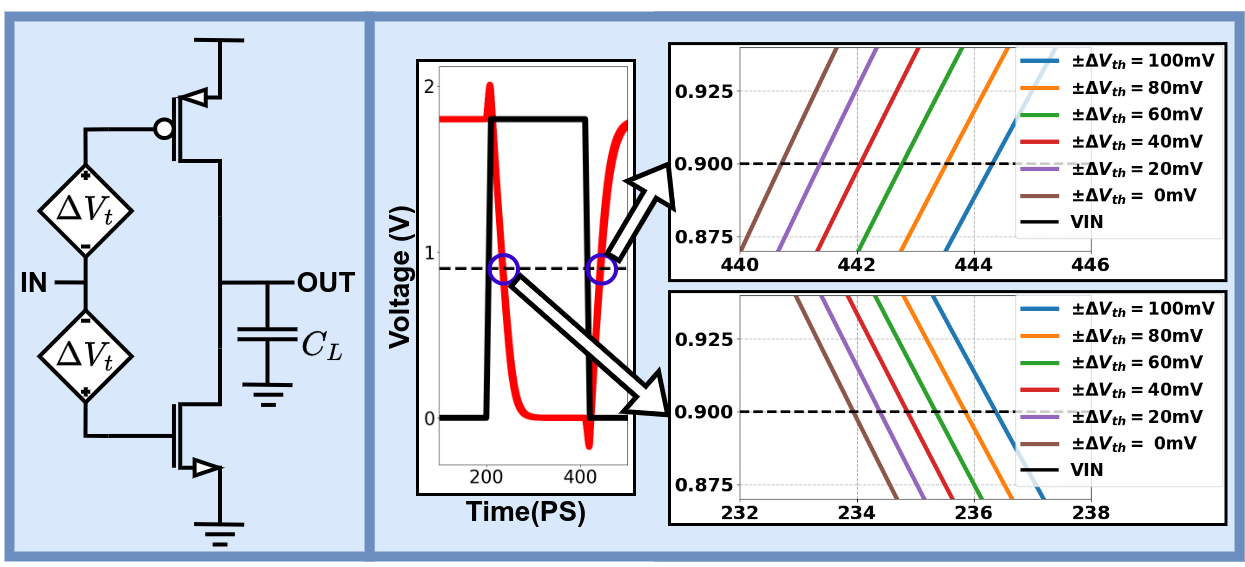
\includegraphics[width=0.9\linewidth]{img/inv_bti.png}
  \caption{Ngspice simulation of SkyWater 130nm inverter high-low/low-high transitions with varied $\Delta V_{th}$. Two voltage sources are placed in series with both NMOS and PMOS gate terminals to model threshold voltage fluctuations. The sources are incremented by 20mV. The output curves with respect to each threshold voltage increment are provided. The shift in output voltage demonstrates the relationship between $\Delta V_{th}$ and $t_p$. For BTI-scale voltage fluctuations, several picoseconds of propagation delay variation are observed. \label{fig:bti_inv}}
\end{figure} 